\documentclass[10pt,twocolumn,letterpaper]{article}

\usepackage{times}
\usepackage{graphicx}
\usepackage{amsmath,amssymb}
\usepackage{booktabs}
\usepackage{microtype}
\usepackage{url}
\usepackage[numbers,sort&compress]{natbib}
\usepackage[breaklinks=true,colorlinks,bookmarks=false]{hyperref}

\renewcommand{\topfraction}{0.9}
\renewcommand{\textfraction}{0.1}
\renewcommand{\floatpagefraction}{0.8}

% GPU-only assets are included only when they were measured (see scripts/sync_paper_assets.py).
\newcommand{\optionalinput}[1]{\IfFileExists{#1.tex}{\input{#1}}{}}
\newcommand{\optionalfigure}[2][]{\IfFileExists{#2}{\includegraphics[#1]{#2}}{}}

% Generated by scripts/generate_report.py from results tables. Do not edit by hand.
\newcommand{\NumCategories}{7}
\newcommand{\NumSeeds}{3}
\newcommand{\NumRuns}{63}
\newcommand{\CalibFraction}{20\%}
\newcommand{\PrimaryBudget}{5}
\newcommand{\PrimaryCostRatio}{10}
\newcommand{\DeploymentPrior}{0.01}
\newcommand{\NumSplits}{20}
\newcommand{\BootstrapB}{2000}
\newcommand{\NumConditions}{18}
\newcommand{\MinTestNominal}{20}
\newcommand{\MaxTestNominal}{58}
\newcommand{\CoarsestResolution}{50}
\newcommand{\MinCalibNominal}{42}
\newcommand{\MaxCalibNominal}{78}
\newcommand{\BudgetViolationShare}{60\%}
\newcommand{\MeanAUROCPatchCore}{0.992}
\newcommand{\MeanAUPROPatchCore}{0.928}
\newcommand{\CCTCostChangePatchCore}{-51\%}
\newcommand{\CCTViolationPatchCore}{10\%}
\newcommand{\NominalViolationPatchCore}{28\%}
\newcommand{\MeanAUROCPaDiM}{0.930}
\newcommand{\MeanAUPROPaDiM}{0.914}
\newcommand{\CCTCostChangePaDiM}{-10\%}
\newcommand{\CCTViolationPaDiM}{29\%}
\newcommand{\NominalViolationPaDiM}{38\%}
\newcommand{\MeanAUROCAE}{0.647}
\newcommand{\MeanAUPROAE}{0.590}
\newcommand{\CCTCostChangeAE}{-10\%}
\newcommand{\CCTViolationAE}{18\%}
\newcommand{\NominalViolationAE}{26\%}
\newcommand{\CoresetSpeedup}{8\ensuremath{\times}}
\newcommand{\CoresetN}{100,000}
\newcommand{\CoresetAgreement}{92.8\%}
\newcommand{\HasLatency}{1}
\newcommand{\HasCoreset}{1}


\title{What MVTec AD Can and Cannot Tell Us About Deployment:\\
Operating Points, Alarm Budgets and Cost-Calibrated Thresholds\\
for Unsupervised Industrial Anomaly Detection}
\author{Utkarsh Sengar\\{\tt\small sengarutkarsh@gmail.com}}

\begin{document}
\maketitle

\begin{abstract}
Image AUROC and AU-PRO rank anomaly detectors without fixing a decision threshold, yet an inspection line
runs at one threshold, under an operator alarm budget, with missed defects far costlier than false alarms.
We evaluate PatchCore-style, PaDiM-style and autoencoder detectors on \NumCategories{} MVTec AD categories
($\NumRuns$ runs, \NumSeeds{} seeds) at fixed operating points. Thresholds are calibrated only on held-out
nominal training images, and every realised rate is reported with an exact interval and with the resolution
the test set allows. Three findings follow. First, MVTec AD test sets contain \MinTestNominal--\MaxTestNominal{}
nominal images, so a budget of \PrimaryBudget{} false alarms per 1,000 parts cannot be verified: the
coarsest category resolves only \CoarsestResolution{} per 1,000. Second, thresholds calibrated on held-out
training images transfer poorly: the realised test false-alarm rate exceeds the \PrimaryBudget/1k target in
\BudgetViolationShare{} of run--category evaluations. Third, cost-calibrated thresholding (CCT), i.e.\
constrained empirical risk minimisation using a few labelled defects, changes expected cost by
\CCTCostChangePatchCore{} (PatchCore), \CCTCostChangePaDiM{} (PaDiM) and \CCTCostChangeAE{} (autoencoder)
relative to a nominal-only budget threshold out of sample, differences that categories-as-units tests cannot
distinguish from zero. Code, score archives and every table are generated by a single pipeline.
\end{abstract}

\section{Introduction}
Benchmarks for unsupervised visual anomaly detection report threshold-free ranking metrics: image-level
AUROC and the per-region-overlap curve integrated up to a 30\% false-positive rate
(AU-PRO)~\cite{bergmann2019mvtec,bergmann2020uninformed,bergmann2021mvtec}. A deployed inspector instead
commits to a threshold. Two constraints then dominate: human reviewers can absorb only a few false alarms per
thousand parts, and an escaped defect costs many times more than a false alarm~\cite{elkan2001foundations}.
This paper asks which statements about such operating points the standard MVTec AD protocol can support.

We make three contributions. (i) A threshold protocol that never touches the test set: thresholds are
calibrated on a held-out 20\% of the nominal training images, and every realised test rate is reported with a
Clopper--Pearson interval~\cite{clopper1934use} and with the resolution the test set permits. (ii) An
out-of-sample evaluation of cost-calibrated thresholding with repeated stratified splits. (iii) Statistical
comparisons that treat categories, not seeds, as the independent units~\cite{demsar2006statistical}, which
makes explicit how little significance seven categories can carry.

\section{Setup}
\paragraph{Data.} We use \NumCategories{} MVTec AD categories (bottle, cable, carpet, grid, hazelnut, leather,
metal nut). Every category is checked against the official per-split, per-defect-type image counts before
use. Images are resized to $256\times256$. For each seed, \CalibFraction{} of \texttt{train/good} is held out
as a nominal calibration set (\MinCalibNominal--\MaxCalibNominal{} images per category); models are fitted on
the rest.

\paragraph{Detectors.} We reimplement PatchCore~\cite{roth2022towards} and PaDiM~\cite{defard2021padim} with an
ImageNet ResNet-18 backbone, and train a convolutional autoencoder from scratch. PatchCore keeps a 10\%
memory bank selected by exact greedy k-center~\cite{sener2018active} in a random 128-d projection; PaDiM fits
per-location Gaussians on 100 random channels. All three produce a pixel map, smoothed with $\sigma=4$, and
use its maximum as the image score. The seed changes the calibration split, PatchCore's projection and start
point, PaDiM's channel subset and the autoencoder's initialisation. These are reimplementations under one
protocol, not reproductions of the published numbers.

\paragraph{Metrics.} AU-PRO is computed exactly at every distinct score following the MVTec protocol. For
robustness we apply 6 corruption types at 3 severities (\NumConditions{} conditions) after resizing, in the spirit
of~\cite{hendrycks2019benchmarking}, and report the non-negative mean robustness degradation (MRD) and the
signed mean change (MPC). A part is flagged when its score is at least $\tau$. With false-alarm cost 1,
missed-defect cost $r$ and production defect rate $\pi$, the expected cost per part is
\begin{equation}
C(\tau) = (1-\pi)\,\mathrm{FPR}(\tau) + \pi\, r\, \mathrm{FNR}(\tau).
\end{equation}
We use $\pi=\DeploymentPrior$ and $r=\PrimaryCostRatio$ unless stated otherwise, and this is the only cost
definition in the paper.

\paragraph{Thresholds.} The \emph{nominal-only budget} rule picks the lowest $\tau$ whose false-positive rate on
the calibration nominals is at most $b/1000$. \emph{CCT} minimises $C(\tau)$ on labelled calibration data,
optionally subject to the same budget. Because CCT needs defects, it is evaluated with \NumSplits{} stratified
50/50 splits of each run's test set: thresholds use one half plus the held-out nominals; metrics use the other
half. An \emph{oracle} that picks the cost-optimal threshold on the evaluation half itself gives a lower bound.

\paragraph{Statistics.} Per-category intervals use a two-stage bootstrap over seeds and test images
($B=\BootstrapB$)~\cite{efron1993introduction}. Method and rule comparisons use two-sided Wilcoxon signed-rank
tests~\cite{wilcoxon1945individual} with one value per category, adjusted with Holm's
procedure~\cite{holm1979simple}. With $n$ categories the smallest attainable $p$-value is $2/2^n$.

\section{Results}
\begin{table}[tbp]
\centering
\small
\caption{Clean test results on 7 MVTec AD categories. Per category: mean $\pm$ std over 3 seeds (seeds change the train/calibration split, PatchCore's projection and start point, PaDiM's channel subset and the autoencoder's initialisation). \textit{Mean} rows: mean $\pm$ std over categories. AU-PRO is integrated up to FPR $=0.3$ with the exact MVTec protocol.}
\label{tab:main_results}
\begin{adjustbox}{max width=\linewidth}
\begin{tabular}{llccc}
\toprule
\textbf{Category} & \textbf{Method} & \textbf{Image AUROC} & \textbf{Pixel AUROC} & \textbf{AU-PRO} \\
\midrule
Bottle & PatchCore & $1.000 \pm 0.000$ & $0.983 \pm 0.000$ & $0.933 \pm 0.001$ \\
Bottle & PaDiM & $0.997 \pm 0.001$ & $0.984 \pm 0.001$ & $0.950 \pm 0.001$ \\
Bottle & ConvAutoencoder & $0.784 \pm 0.008$ & $0.735 \pm 0.004$ & $0.530 \pm 0.003$ \\
\midrule
Cable & PatchCore & $0.991 \pm 0.002$ & $0.985 \pm 0.000$ & $0.940 \pm 0.002$ \\
Cable & PaDiM & $0.855 \pm 0.008$ & $0.971 \pm 0.003$ & $0.905 \pm 0.005$ \\
Cable & ConvAutoencoder & $0.336 \pm 0.008$ & $0.617 \pm 0.055$ & $0.406 \pm 0.010$ \\
\midrule
Carpet & PatchCore & $0.986 \pm 0.000$ & $0.990 \pm 0.000$ & $0.935 \pm 0.002$ \\
Carpet & PaDiM & $0.964 \pm 0.005$ & $0.987 \pm 0.000$ & $0.943 \pm 0.004$ \\
Carpet & ConvAutoencoder & $0.335 \pm 0.025$ & $0.735 \pm 0.020$ & $0.417 \pm 0.013$ \\
\midrule
Grid & PatchCore & $0.968 \pm 0.004$ & $0.977 \pm 0.002$ & $0.902 \pm 0.005$ \\
Grid & PaDiM & $0.862 \pm 0.050$ & $0.926 \pm 0.011$ & $0.832 \pm 0.050$ \\
Grid & ConvAutoencoder & $0.850 \pm 0.044$ & $0.818 \pm 0.026$ & $0.620 \pm 0.040$ \\
\midrule
Hazelnut & PatchCore & $1.000 \pm 0.000$ & $0.987 \pm 0.000$ & $0.881 \pm 0.005$ \\
Hazelnut & PaDiM & $0.858 \pm 0.010$ & $0.981 \pm 0.002$ & $0.869 \pm 0.003$ \\
Hazelnut & ConvAutoencoder & $0.981 \pm 0.003$ & $0.978 \pm 0.003$ & $0.874 \pm 0.013$ \\
\midrule
Leather & PatchCore & $1.000 \pm 0.000$ & $0.992 \pm 0.000$ & $0.973 \pm 0.000$ \\
Leather & PaDiM & $0.999 \pm 0.001$ & $0.994 \pm 0.001$ & $0.982 \pm 0.004$ \\
Leather & ConvAutoencoder & $0.860 \pm 0.005$ & $0.968 \pm 0.007$ & $0.933 \pm 0.005$ \\
\midrule
Metal Nut & PatchCore & $0.997 \pm 0.001$ & $0.984 \pm 0.000$ & $0.935 \pm 0.001$ \\
Metal Nut & PaDiM & $0.973 \pm 0.004$ & $0.972 \pm 0.005$ & $0.916 \pm 0.006$ \\
Metal Nut & ConvAutoencoder & $0.383 \pm 0.012$ & $0.671 \pm 0.009$ & $0.349 \pm 0.022$ \\
\midrule
\textit{Mean} & PatchCore & $0.992 \pm 0.012$ & $0.985 \pm 0.005$ & $0.928 \pm 0.029$ \\
\textit{Mean} & PaDiM & $0.930 \pm 0.068$ & $0.974 \pm 0.022$ & $0.914 \pm 0.051$ \\
\textit{Mean} & ConvAutoencoder & $0.647 \pm 0.283$ & $0.789 \pm 0.140$ & $0.590 \pm 0.233$ \\
\bottomrule
\end{tabular}
\end{adjustbox}
\end{table}


\paragraph{Ranking metrics.} Table~\ref{tab:main_results} reproduces the familiar ordering: PatchCore-style
(mean image AUROC \MeanAUROCPatchCore, AU-PRO \MeanAUPROPatchCore) ahead of PaDiM-style (\MeanAUROCPaDiM,
\MeanAUPROPaDiM) and the autoencoder (\MeanAUROCAE, \MeanAUPROAE). Table~\ref{tab:robustness} and
Fig.~\ref{fig:robustness} show the corruption sensitivity of the feature-based detectors.

\begin{table}[tbp]
\centering
\small
\caption{Robustness over 18 corruption conditions (6 types $\times$ 3 severities, applied after resizing to 256 px). MRD $=\frac{1}{18}\sum_i\max(0,M_{clean}-M_i)$; MPC is the signed mean. Values are means over 3 seeds.}
\label{tab:robustness}
\begin{adjustbox}{max width=\linewidth}
\begin{tabular}{llccc}
\toprule
\textbf{Category} & \textbf{Method} & \textbf{MRD (AUROC)} $\downarrow$ & \textbf{MRD (AU-PRO)} $\downarrow$ & \textbf{MPC (AUROC)} \\
\midrule
Bottle & PatchCore & 0.057 & 0.108 & $+0.057$ \\
Bottle & PaDiM & 0.179 & 0.234 & $+0.179$ \\
Bottle & ConvAutoencoder & 0.115 & 0.208 & $+0.105$ \\
\midrule
Cable & PatchCore & 0.171 & 0.144 & $+0.171$ \\
Cable & PaDiM & 0.123 & 0.195 & $+0.119$ \\
Cable & ConvAutoencoder & 0.001 & 0.068 & $-0.075$ \\
\midrule
Carpet & PatchCore & 0.106 & 0.146 & $+0.106$ \\
Carpet & PaDiM & 0.248 & 0.279 & $+0.247$ \\
Carpet & ConvAutoencoder & 0.005 & 0.085 & $-0.121$ \\
\midrule
Grid & PatchCore & 0.327 & 0.485 & $+0.327$ \\
Grid & PaDiM & 0.295 & 0.390 & $+0.295$ \\
Grid & ConvAutoencoder & 0.244 & 0.133 & $+0.243$ \\
\midrule
Hazelnut & PatchCore & 0.049 & 0.073 & $+0.049$ \\
Hazelnut & PaDiM & 0.102 & 0.217 & $+0.078$ \\
Hazelnut & ConvAutoencoder & 0.044 & 0.095 & $+0.043$ \\
\midrule
Leather & PatchCore & 0.056 & 0.067 & $+0.056$ \\
Leather & PaDiM & 0.143 & 0.099 & $+0.143$ \\
Leather & ConvAutoencoder & 0.060 & 0.100 & $+0.053$ \\
\midrule
Metal Nut & PatchCore & 0.168 & 0.190 & $+0.168$ \\
Metal Nut & PaDiM & 0.224 & 0.345 & $+0.222$ \\
Metal Nut & ConvAutoencoder & 0.003 & 0.031 & $-0.092$ \\
\midrule
\textit{Mean} & PatchCore & 0.133 & 0.173 & $+0.133$ \\
\textit{Mean} & PaDiM & 0.188 & 0.251 & $+0.183$ \\
\textit{Mean} & ConvAutoencoder & 0.067 & 0.103 & $+0.022$ \\
\bottomrule
\end{tabular}
\end{adjustbox}
\end{table}


\begin{figure*}[t]
\centering
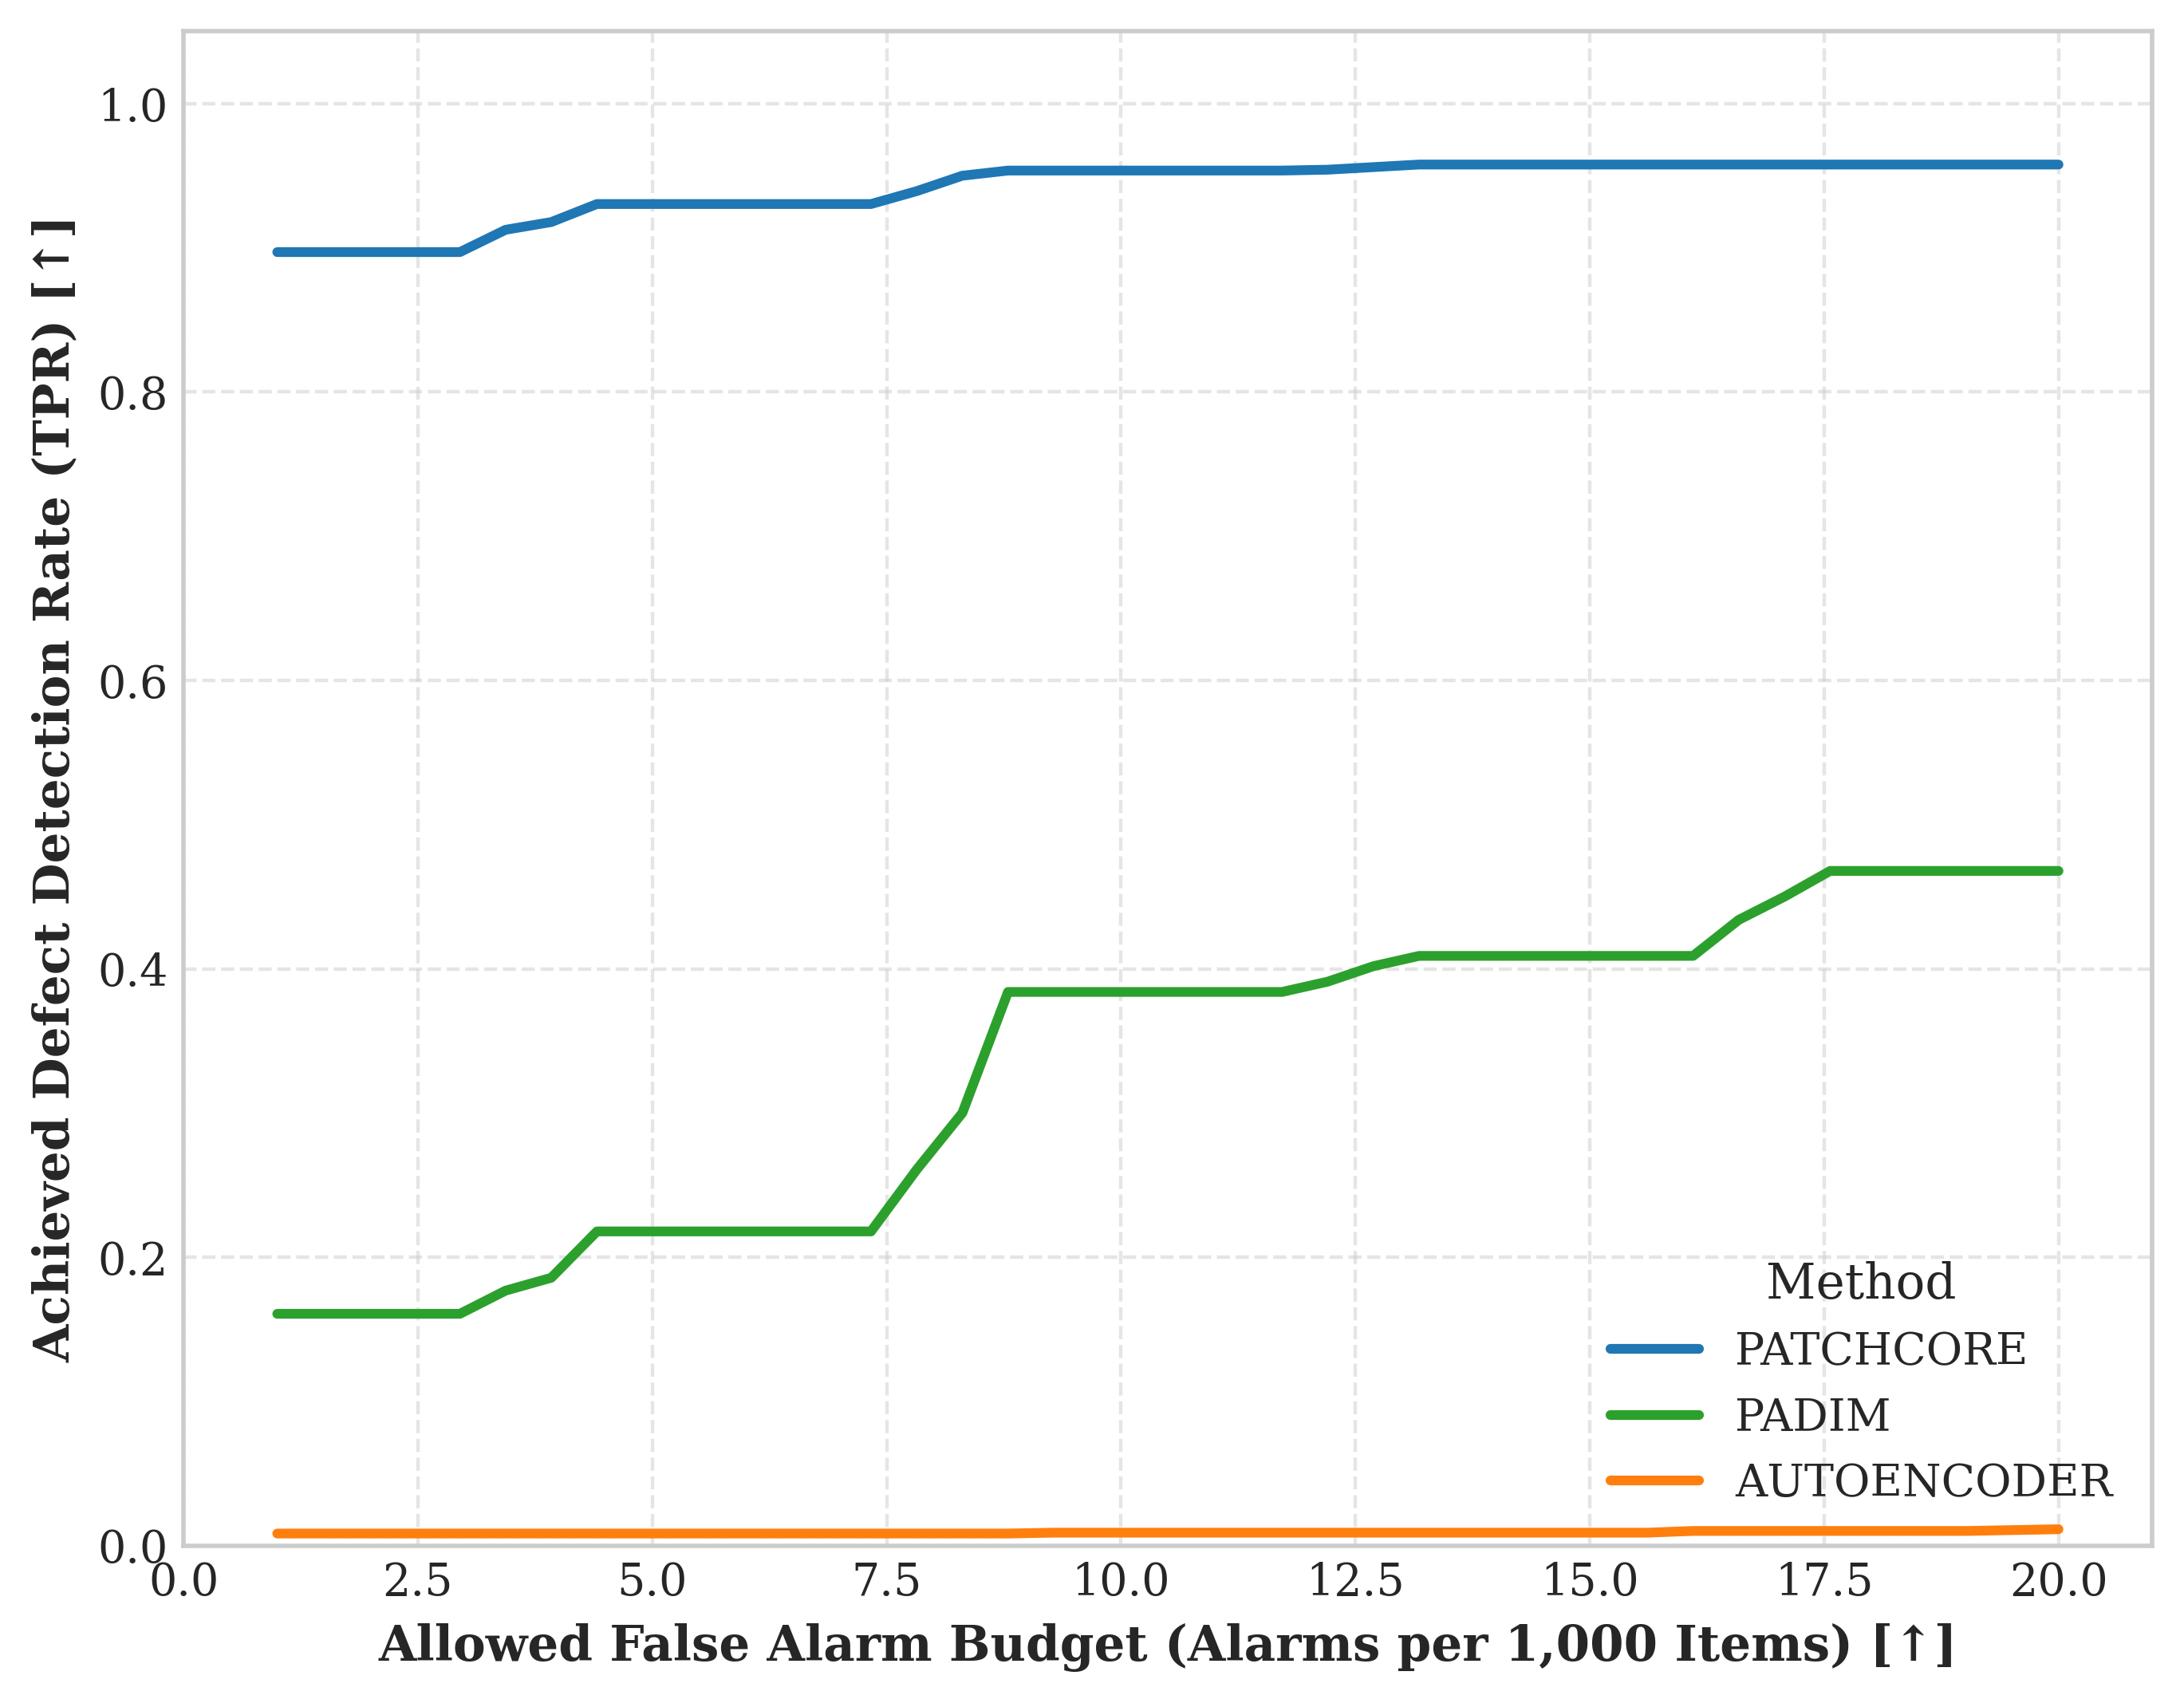
\includegraphics[width=0.32\linewidth]{figures/tpr_vs_alert_budget.png}\hfill
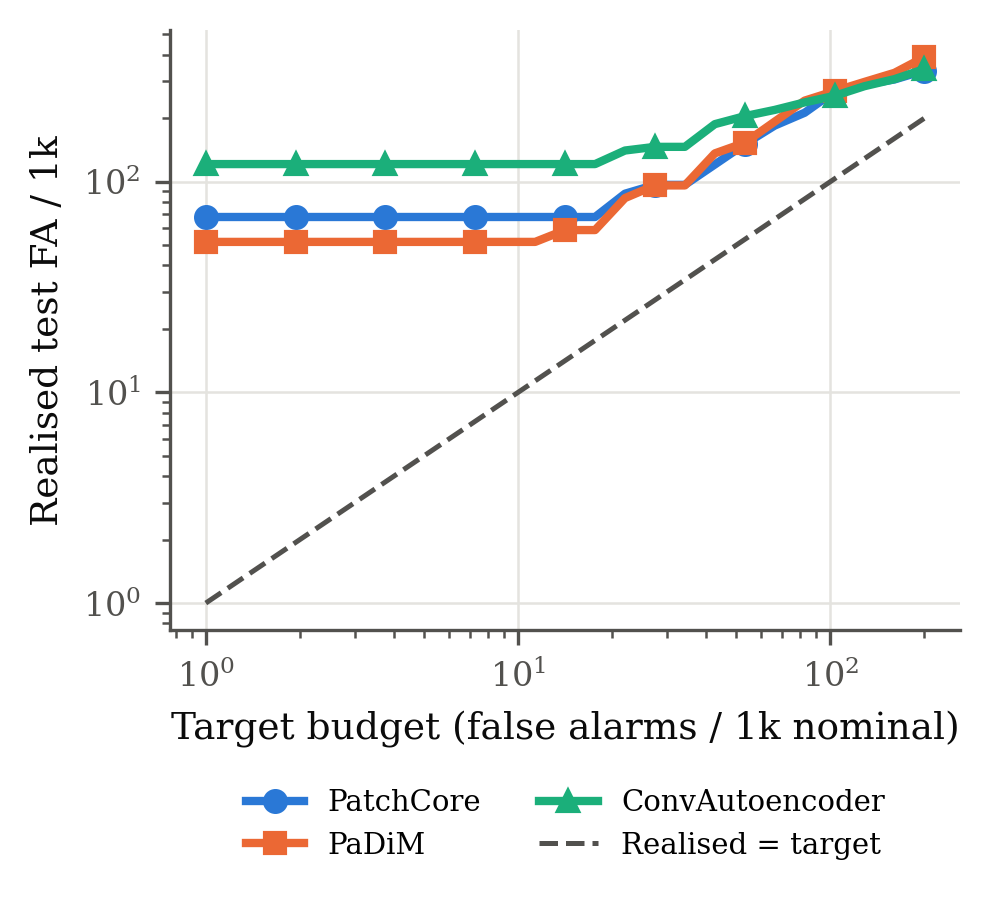
\includegraphics[width=0.32\linewidth]{figures/realized_vs_target_alarms.png}\hfill
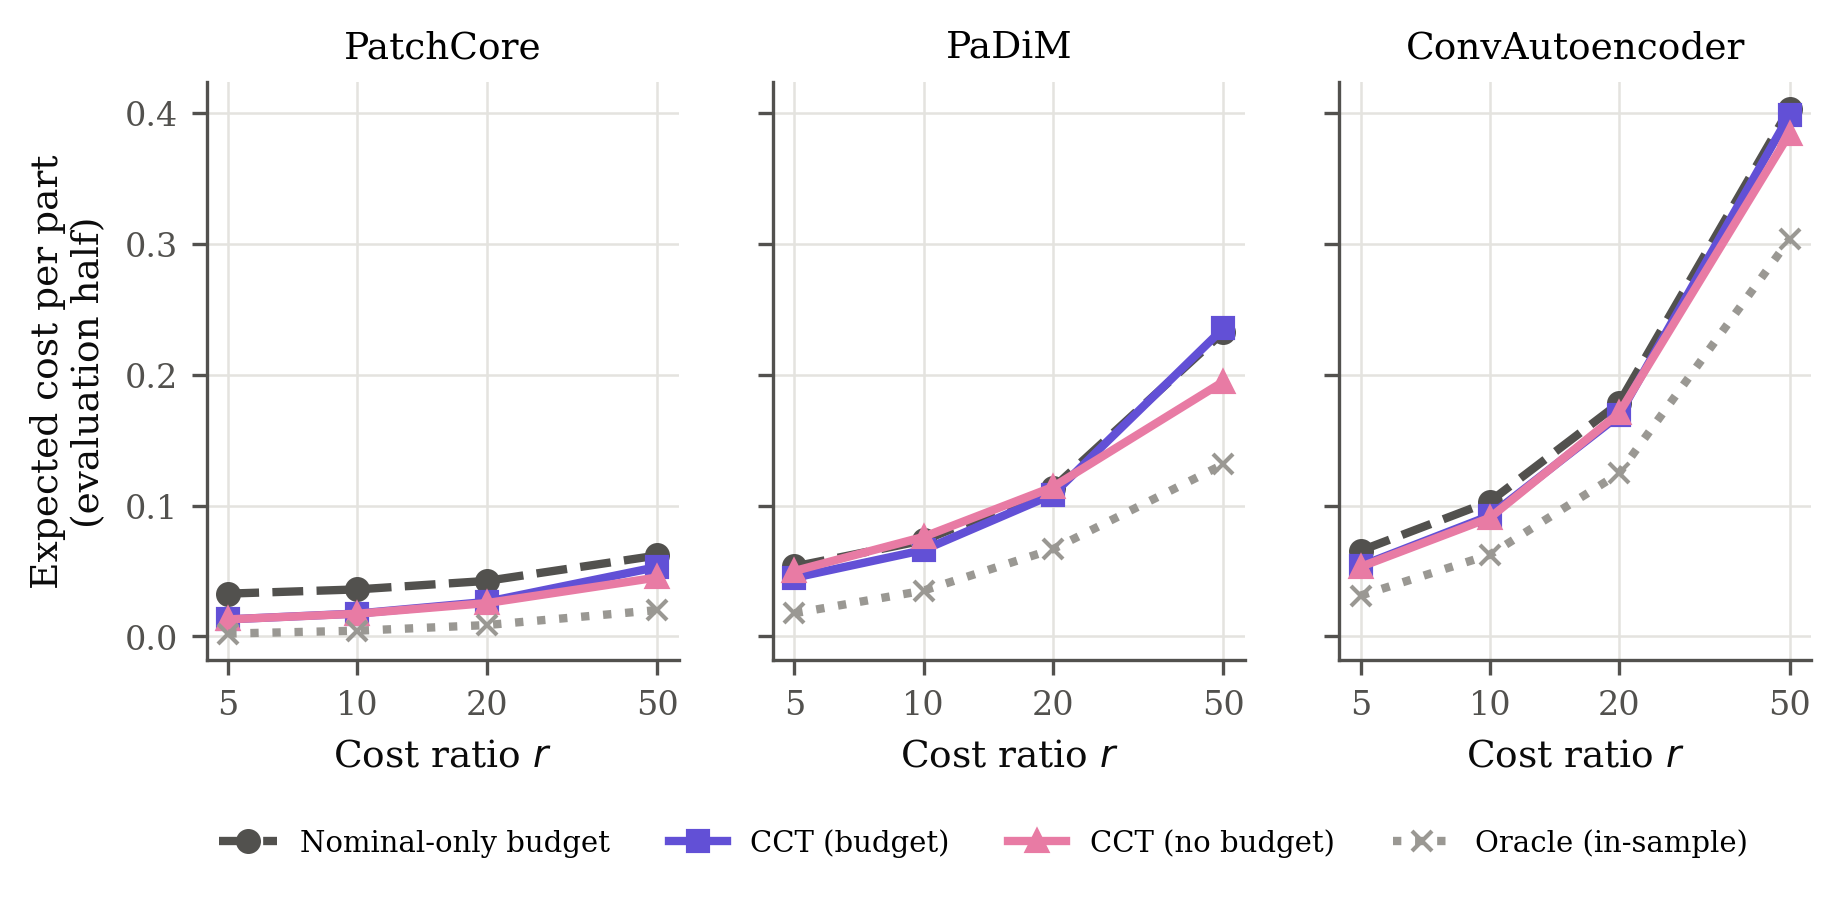
\includegraphics[width=0.34\linewidth]{figures/cct_cost_vs_ratio.png}
\caption{Left: test defect recall when the threshold is calibrated on held-out nominal training images for a
target budget (macro-average over categories; band: range over categories). Centre: realised test false-alarm
rate against the target; the dashed line marks equality. Rates below the test-set resolution cannot be
observed. Right: out-of-sample expected cost of each threshold rule as the cost ratio grows.}
\label{fig:operating}
\end{figure*}

\paragraph{Operating points.} Table~\ref{tab:operational} and Fig.~\ref{fig:operating} report the operating point
at a target of \PrimaryBudget{} false alarms per 1,000 nominal parts. Two effects limit what can be claimed.
The test sets are too small to observe rates of this size: one false alarm on the smallest nominal set already
amounts to \CoarsestResolution{} per 1,000. And the calibration images do not represent the nominal test images
well, so realised test false-alarm rates exceed the target in \BudgetViolationShare{} of evaluations
(Fig.~\ref{fig:operating}, centre). A threshold that satisfies an alarm budget on training-distribution
nominals is therefore no guarantee on the test distribution, and per-mille budgets need far larger nominal
validation sets than MVTec AD provides.

\begin{table}[tbp]
\centering
\small
\caption{Operating point at a target budget of 5 false alarms per 1,000 nominal parts. The threshold is set on held-out train/good images only (42--78 per category) and applied to the full test set. Brackets: 95\% two-stage bootstrap intervals over seeds and test images ($B=2000$). ``Resolution'' is the smallest non-zero rate the test set can express (1000 / nominal test images). Expected cost uses defect prior $\pi=0.01$ and cost ratio $r=10$.}
\label{tab:operational}
\begin{adjustbox}{max width=\linewidth}
\begin{tabular}{llcccc}
\toprule
\textbf{Category} & \textbf{Method} & \textbf{Test TPR} & \textbf{Test FA/1k} & \textbf{Resolution/1k} & \textbf{Exp. cost} \\
\midrule
Bottle & PatchCore & 1.000 [1.000, 1.000] & 0.0 [0.0, 0.0] & 50.0 & 0.0000 \\
Bottle & PaDiM & 0.937 [0.889, 0.974] & 33.3 [0.0, 100.0] & 50.0 & 0.0393 \\
Bottle & ConvAutoencoder & 0.444 [0.296, 0.603] & 16.7 [0.0, 66.7] & 50.0 & 0.0721 \\
\midrule
Cable & PatchCore & 0.866 [0.797, 0.924] & 0.0 [0.0, 0.0] & 17.2 & 0.0134 \\
Cable & PaDiM & 0.243 [0.134, 0.388] & 23.0 [0.0, 63.2] & 17.2 & 0.0985 \\
Cable & ConvAutoencoder & 0.007 [0.000, 0.022] & 34.5 [0.0, 86.2] & 17.2 & 0.1334 \\
\midrule
Carpet & PatchCore & 0.978 [0.955, 0.996] & 309.5 [154.8, 500.3] & 35.7 & 0.3087 \\
Carpet & PaDiM & 0.835 [0.738, 0.925] & 59.5 [0.0, 142.9] & 35.7 & 0.0754 \\
Carpet & ConvAutoencoder & 0.079 [0.030, 0.131] & 190.5 [71.4, 321.4] & 35.7 & 0.2807 \\
\midrule
Grid & PatchCore & 0.860 [0.801, 0.912] & 47.6 [0.0, 111.1] & 47.6 & 0.0612 \\
Grid & PaDiM & 0.316 [0.193, 0.450] & 15.9 [0.0, 63.5] & 47.6 & 0.0841 \\
Grid & ConvAutoencoder & 0.006 [0.000, 0.023] & 0.0 [0.0, 0.0] & 47.6 & 0.0994 \\
\midrule
Hazelnut & PatchCore & 0.967 [0.938, 0.990] & 0.0 [0.0, 0.0] & 25.0 & 0.0033 \\
Hazelnut & PaDiM & 0.533 [0.352, 0.781] & 108.3 [33.3, 208.3] & 25.0 & 0.1539 \\
Hazelnut & ConvAutoencoder & 0.586 [0.376, 0.738] & 0.0 [0.0, 0.0] & 25.0 & 0.0414 \\
\midrule
Leather & PatchCore & 1.000 [1.000, 1.000] & 72.9 [20.8, 135.4] & 31.2 & 0.0722 \\
Leather & PaDiM & 0.993 [0.978, 1.000] & 31.2 [0.0, 83.3] & 31.2 & 0.0317 \\
Leather & ConvAutoencoder & 0.859 [0.808, 0.906] & 500.0 [375.0, 614.6] & 31.2 & 0.5091 \\
\midrule
Metal Nut & PatchCore & 0.975 [0.953, 0.993] & 45.5 [0.0, 121.2] & 45.5 & 0.0475 \\
Metal Nut & PaDiM & 0.910 [0.864, 0.957] & 90.9 [15.2, 197.0] & 45.5 & 0.0990 \\
Metal Nut & ConvAutoencoder & 0.029 [0.011, 0.050] & 106.1 [30.3, 197.0] & 45.5 & 0.2021 \\
\bottomrule
\end{tabular}
\end{adjustbox}
\end{table}


\paragraph{Cost-calibrated thresholds.} Table~\ref{tab:cct} compares threshold rules out of sample. Using
labelled calibration defects changes the expected cost by \CCTCostChangePatchCore, \CCTCostChangePaDiM{} and
\CCTCostChangeAE{} for the three detectors. Budget violations on the evaluation halves occur for every rule
(nominal-only: \NominalViolationPatchCore, \NominalViolationPaDiM, \NominalViolationAE; CCT with budget:
\CCTViolationPatchCore, \CCTViolationPaDiM, \CCTViolationAE). The gap to the in-sample oracle is larger than the
difference between deployable rules, which says that the main limitation is the amount of calibration data, not
the choice of rule. With \NumCategories{} categories as units, none of the comparisons can be declared
significant after Holm adjustment unless all categories agree in sign.

\begin{table}[tbp]
\centering
\small
\caption{Out-of-sample threshold selection, cost ratio $r=10$, prior $\pi=0.01$, budget 5/1k. Each run's test set is split 50/50 (stratified) 20 times; thresholds use the calibration half plus held-out train/good nominals; metrics are measured on the other half. Cost: mean $\pm$ std over categories (each category averaged over seeds and splits). ``Violations'': share of evaluations whose realised FA/1k exceeds the budget. $p$: Holm-adjusted two-sided Wilcoxon signed-rank test against the nominal-only budget rule with categories as units ($n=7$, smallest attainable $p=0.016$ before adjustment).}
\label{tab:cct}
\begin{adjustbox}{max width=\linewidth}
\begin{tabular}{llcccc}
\toprule
\textbf{Method} & \textbf{Rule} & \textbf{Expected cost} & \textbf{FA/1k} & \textbf{Violations} & \textbf{$p$ (Holm)} \\
\midrule
PatchCore & Nominal-only budget & $0.0359 \pm 0.0300$ & 29.7 & 28\% &  \\
PatchCore & CCT (budget) & $0.0175 \pm 0.0231$ & 8.6 & 10\% & 1.000 \\
PatchCore & CCT (no budget) & $0.0173 \pm 0.0227$ & 8.6 & 10\% & 1.000 \\
PatchCore & Oracle (in-sample) & $0.0043 \pm 0.0062$ & 0.0 & 0\% &  \\
\midrule
PaDiM & Nominal-only budget & $0.0733 \pm 0.0335$ & 33.9 & 38\% &  \\
PaDiM & CCT (budget) & $0.0660 \pm 0.0433$ & 23.9 & 29\% & 0.875 \\
PaDiM & CCT (no budget) & $0.0761 \pm 0.0566$ & 43.5 & 40\% & 1.000 \\
PaDiM & Oracle (in-sample) & $0.0350 \pm 0.0334$ & 1.4 & 3\% &  \\
\midrule
ConvAutoencoder & Nominal-only budget & $0.1031 \pm 0.0402$ & 28.2 & 26\% &  \\
ConvAutoencoder & CCT (budget) & $0.0922 \pm 0.0286$ & 15.8 & 18\% & 0.781 \\
ConvAutoencoder & CCT (no budget) & $0.0906 \pm 0.0317$ & 16.4 & 18\% & 0.188 \\
ConvAutoencoder & Oracle (in-sample) & $0.0624 \pm 0.0356$ & 0.0 & 0\% &  \\
\bottomrule
\end{tabular}
\end{adjustbox}
\end{table}

\begin{table}[tbp]
\centering
\small
\caption{Paired comparison of expected cost ($r=10$, budget 5/1k) between methods, one value per category (mean over seeds). Two-sided Wilcoxon signed-rank test; Holm adjustment over the three comparisons.}
\label{tab:significance}
\begin{adjustbox}{max width=\linewidth}
\begin{tabular}{lcccc}
\toprule
\textbf{Comparison} & \textbf{$n$} & \textbf{Hodges--Lehmann $\Delta$} & \textbf{$p$} & \textbf{$p$ (Holm)} \\
\midrule
ConvAutoencoder vs PaDiM & 7 & +0.0685 & 0.156 & 0.312 \\
ConvAutoencoder vs PatchCore & 7 & +0.0876 & 0.031 & 0.094 \\
PaDiM vs PatchCore & 7 & +0.0342 & 0.578 & 0.578 \\
\bottomrule
\end{tabular}
\end{adjustbox}
\end{table}


\begin{figure}[t]
\centering
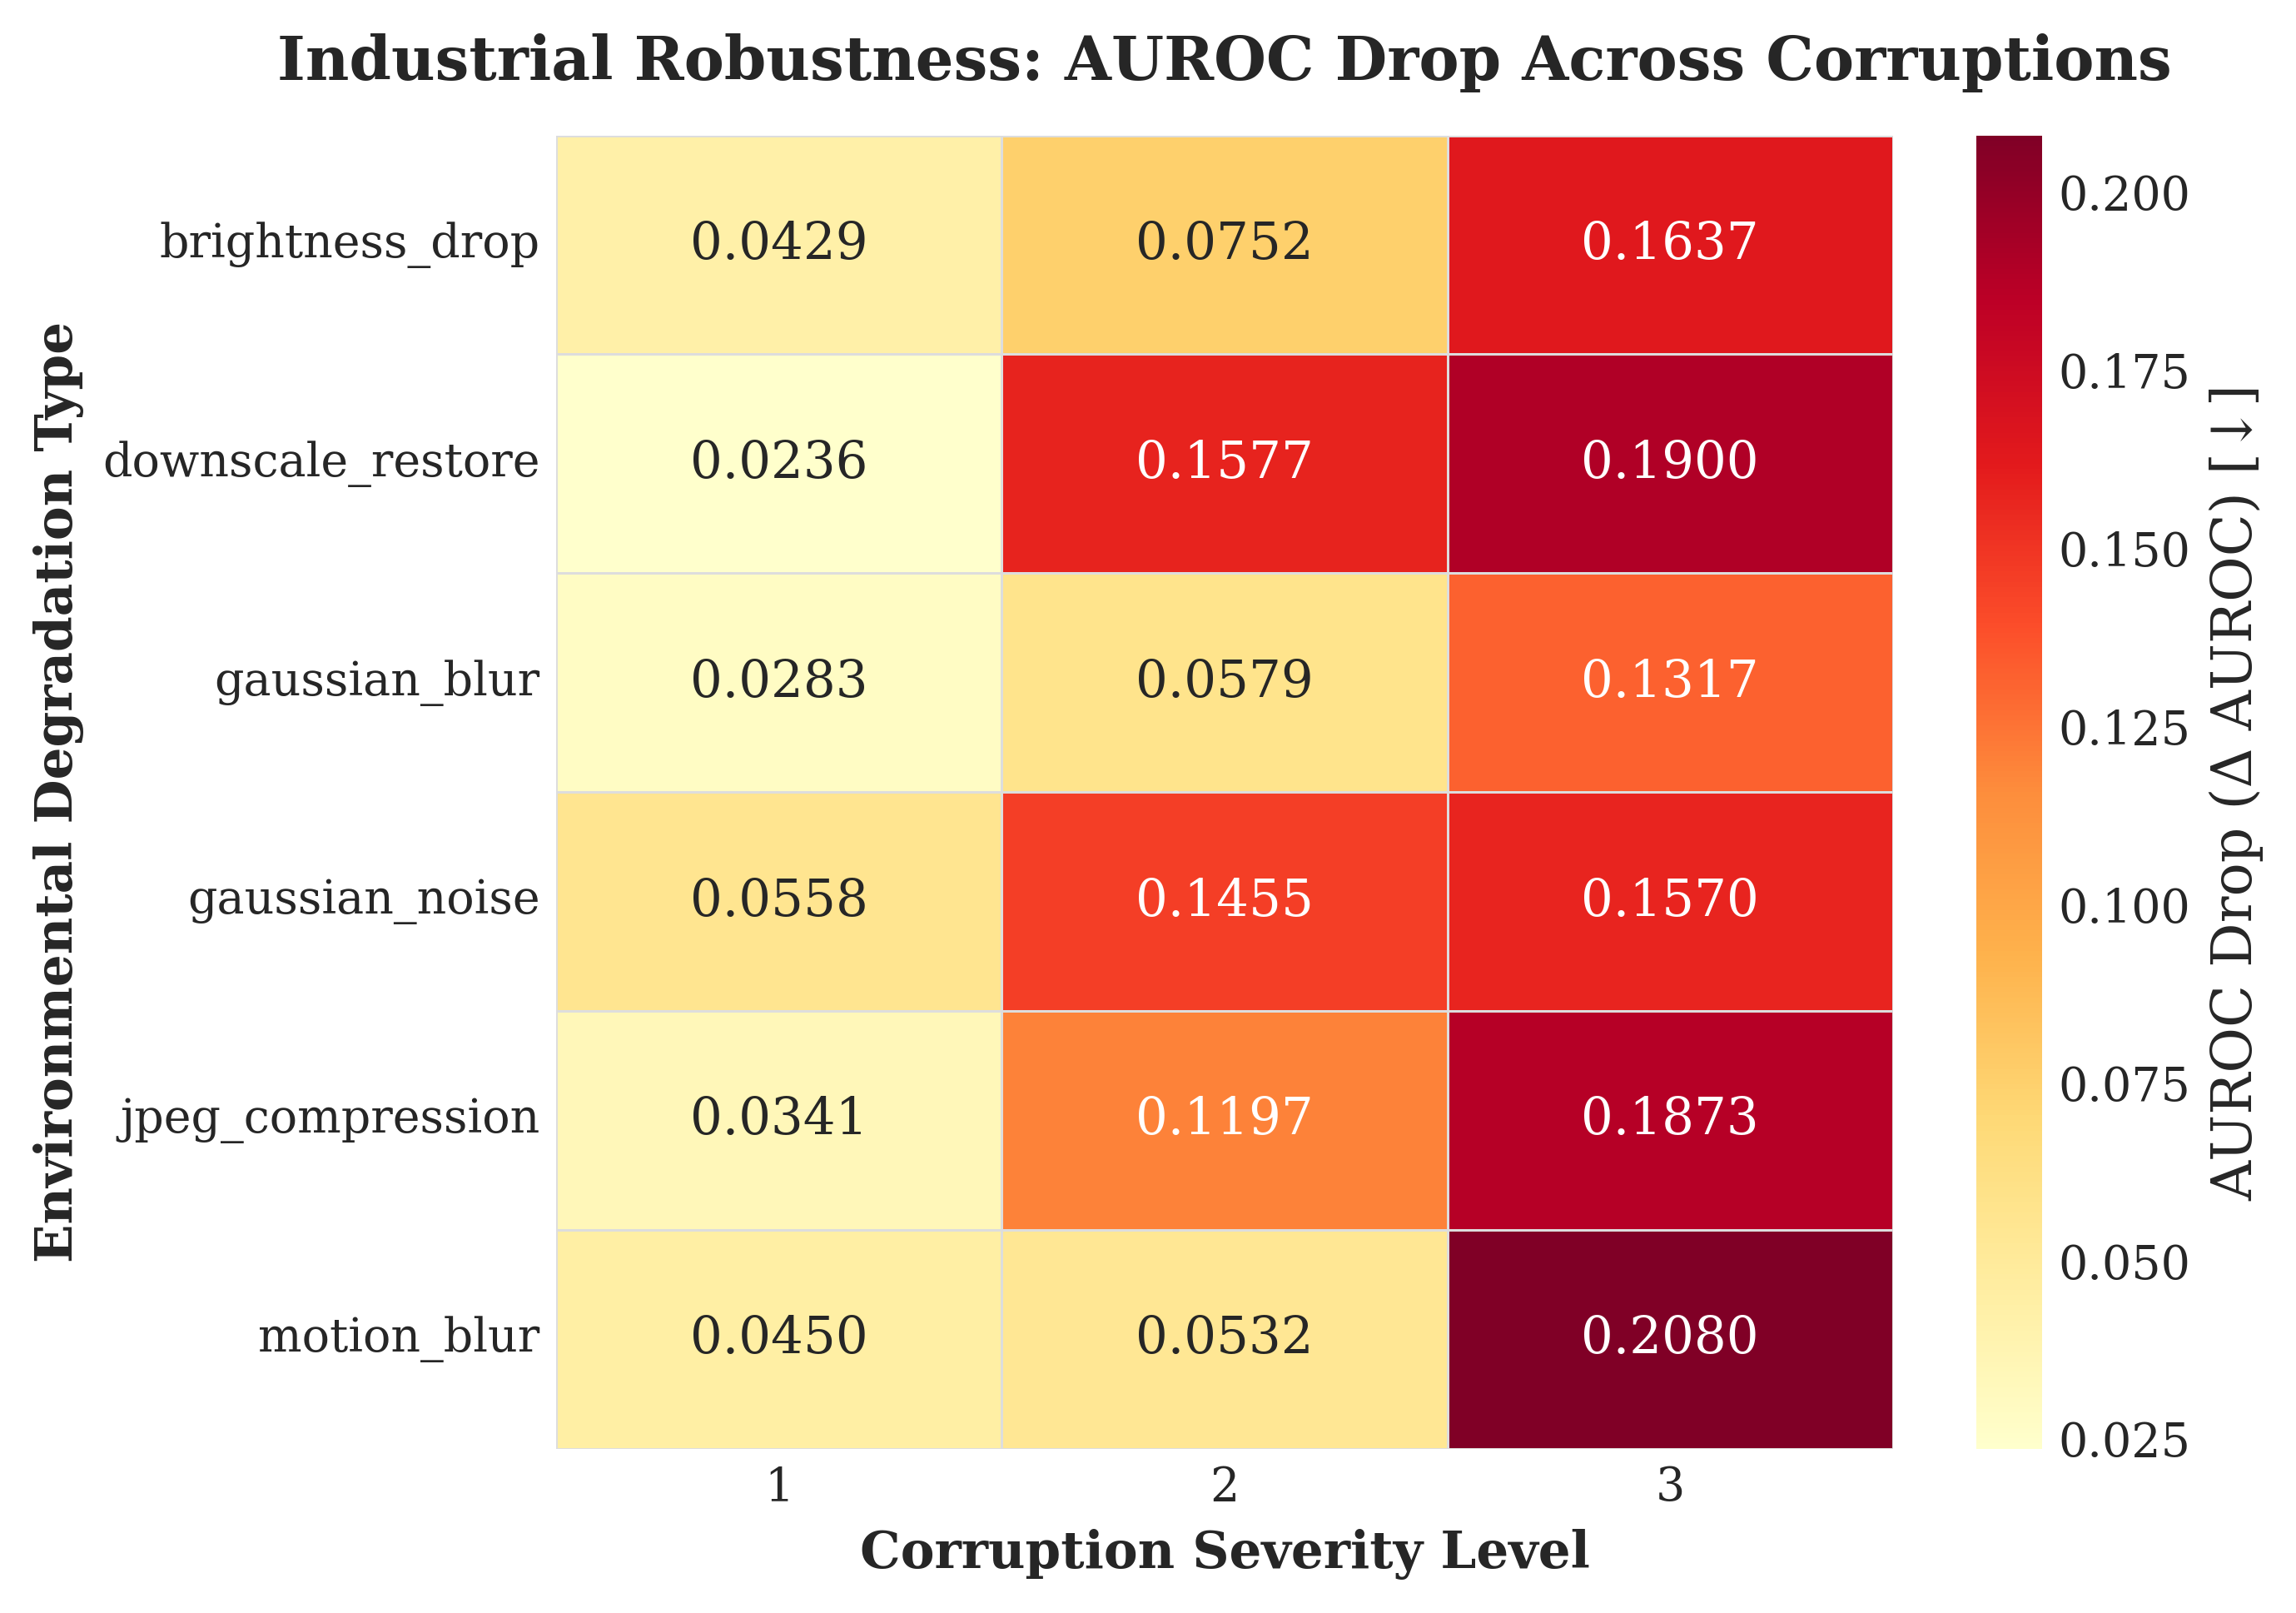
\includegraphics[width=\linewidth]{figures/robustness_heatmap.png}
\caption{Mean drop in image AUROC per corruption and severity (averaged over categories and seeds).}
\label{fig:robustness}
\end{figure}

\optionalinput{tables/latency}
\optionalinput{tables/coreset}

\section{Limitations}
The baselines use ResNet-18 at 256\,px and do not match published PatchCore and PaDiM numbers. Seven
categories bound the strength of any between-method test. The corruptions are synthetic proxies. Operator-load
projections in the accompanying report resample the measured scores and add no information beyond them. The
CCT evaluation draws its labelled defects from the test set, which a real line would have to collect separately.
Latency and the GPU coreset-selection benchmark are reported only when measured on a GPU.

\section{Conclusion}
At deployment-relevant operating points, MVTec AD supports ranking statements but not alarm-budget guarantees:
its nominal test sets are too small to resolve per-mille rates, and nominal training images do not calibrate
thresholds for the test distribution. Cost-calibrated thresholds are cheap to compute and easy to evaluate
honestly, but on this benchmark their benefit cannot be separated from noise. We release the full pipeline so
that each of these statements can be checked and extended to larger nominal validation sets.

{\small
\bibliographystyle{plainnat}
\bibliography{references}
}
\end{document}
